\documentclass{article}
\usepackage{graphicx}
\usepackage{amssymb}
\usepackage{amsmath}

\begin{document}

\title{16-720 Computer Vision: Homework 1}
\author{Xiang Zhi Tan}

\maketitle

\section{Question 1.0}
The first row of filters shown in the figure 3 are gaussian filters. Their role is so smooth out the age such that even with random sampling over the image, we can still collect a general large picture. The second row of filters are lapalsian filters that are edge detectors. The third row of filters are edge detectors on the y-axis. These filter will amplify edges that are vertical. The last rows are edge detectors for the x-axis and highlights edges that are vertical. 

\section{Final Implementation}
The final implementation of the system uses the following variables:
\begin{itemize}
	\item Filter Bank Size,$F = 20$  
	\item Dictionary Size, $K = 300$
	\item $\alpha = 150$
	\item Layer, $L=2$
\end{itemize}
The accuracy of the system on the training set is:$40\%$.
The numeric value of the confusion matrix is as following:

\begin{equation*}
\begin{pmatrix}
    12     &3     &0     &1     &0     &0     &1     &3\\
     5     &7     &1     &0     &4     &2     &1     &0\\
     6     &9     &3     &1     &0     &0     &1     &0\\
     6     &3     &0     &3     &1     &3     &4     &0\\
     1     &0     &1     &1    &13     &0     &3     &1\\
     3     &4     &1     &2     &1     &5     &3     &1\\
     4     &1     &1     &4     &4     &1     &4     &1\\
     0     &0     &1     &1     &1    & 0     &0    &17
\end{pmatrix}
\end{equation*}

\begin{figure}
    \centering
    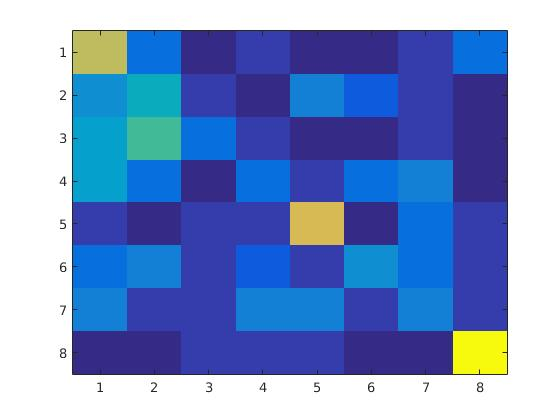
\includegraphics[width=3.0in]{confusion-matrix}
    \caption{Confusion Matrix}
    \label{Confusion Matrix}
\end{figure}

\end{document}